\documentclass[a4paper,10pt]{article}
\usepackage[brazil]{babel}
\usepackage[utf8]{inputenc}
\usepackage[T1]{fontenc}
\usepackage{amsmath}
\usepackage{hyperref}
\usepackage{url}
\usepackage{graphicx}

\title{Relatório Final de Técnica de Programação 1}
\author{
Felipe Luís Pinheiro\footnote{\href{mailto:flpinheiro@gmail.com}{flpinheiro@gmail.com}} - 18/0052667 \and 
Gabriel Teixeira da Silva\footnote{\href{mailto:gabrielbsb21@outlook.com}{gabrielbsb21@outlook.com}} - 170079538 \and 
Paula Vycthória de Araújo Lima\footnote{\href{mailto:araujopaula534@gmail.com}{araujopaula534@gmail.com}} - 170112446 \and 
Rodrigo Belone Ramos\footnote{\href{mailto:rodrigobeloner@gmail.com}{rodrigobeloner@gmail.com}} - 170071804}

\begin{document}

\maketitle

\begin{abstract}
Este relatório faz parte do processo de avaliação da disciplina Técnica de Programação 1 (117889) do Instituto de Ciências Exatas, Departamento de Ciência da Computação da Universidade de Brasília - Brasil, DF, Ministrada pelo professor Cristhian Ivan Riaño Jaimes. 

Neste relatório mostramos o desenvolvimento UML de 4 projetos (Locadora de Carro, Sistema de Cinema, Sistema de Hotelaria e Locadora de Video Game) e por fim desenvolvemos o projeto ... até a sua conclusão como software completamente funcional. 
\end{abstract}

\section{Introdução}

A UML tem origem na compilação das ``melhores práticas de engenharia'' que provaram ter sucesso na modelagem de sistemas grandes e complexos. Sucedeu aos conceitos de Booch, OMT (Rumbaugh) e OOSE (Jacobson) fundindo-os numa única linguagem de modelagem comum e largamente utilizada. A UML pretende ser a linguagem de modelagem padrão para modelar sistemas concorrentes e distribuídos.

A UML ainda não é um padrão da indústria, mas esse objetivo está a tomar forma sob os auspícios do Object Management Group (OMG). O OMG pediu informação acerca de metodologias orientadas a objetos que pudessem criar uma linguagem rigorosa de modelagem de software. Muitos líderes da indústria responderam na esperança de ajudar a criar o padrão. \cite{WebSite:UML}

\section{Projetos}

A seguir mostramos os 4 projetos proposto pelo professor:

\subsection{Locadora de Carro}

Parte 1: Levar em consideração os seguintes requisitos:

\begin{itemize}
	\item A empresa tem muitos automóveis. Cada automóvel tem atributos como numero da placa, cor, ano, tipo de combustível, numero de portas quilometragem, RENAVAM, chassi, valor de locação, etc.
	\item  Cada carro tem um modelo e uma marca, mas o modelo pode relacionar-se a muitos carros, e uma marca pode referir-se a muitos modelos, embora cada modelo só tenha uma marca especifica.
	\item Um carro pode ser alugado por muitos clientes, em momentos diferentes, e um cliente pode alugar muitos carros. É preciso saber quais carros estão locados ou não. Sempre que um carro for locado é preciso armazenar a data e a hora de sua locação e, quando for devolvido, a data e hora de devolução.
\end{itemize}

Parte 2: Uma locadora de carros deseja fazer um sistema para armazenar as informações das
locações que os clientes fazem. A locadora possui varias agencias (código agencia, e localidade).
É necessário registrar tanto a data, hora e agência para cada alocação como para sua devolução e
dados do cliente. A locação pode ser tanto diária (precisa de dias previstos para devolução) como
por período (aplica porcentagem de desconto dado no valor da diária). A locadora armazena
dados dos carros (modelo, placa, cor, ano e data de aquisição) e classifi ca em uma categoria para
definir seu valor de diária de locação

\subsection{Sistema de Cinema}

Requisitos gerais:

\begin{itemize}
	\item Um cinema pode ter muitas salas, sendo necessário, por tanto, registrar informações a respeito de cada uma, como sua capacidade, ou seja, o numero de assentos disponíveis.
	\item O cinema apresenta muitos filmes. Um filme tem informações, titulo e duração. Assim, sempre que um filme for ser apresentado, deve-se registrá-lo também.
	\item Um mesmo filme pode ser apresentado em diferentes salas e em horários diferentes. Cada apresentação em uma determinada sala e horário é chamada sessão. Um filme sendo apresentado em uma sessão tem um conjunto máximo de ingressos, determinado pela capacidade da sala.
	\item Os clientes do cinema podem comprar ou não ingressos para assistir a uma sessão. O
funcionário deve intermediar a compra do ingresso. Um ingresso deve conter informação
como o tipo de ingresso (Meio ingresso ou ingresso inteiro). Além disso, um cliente só pode
comprar ingressos para sessões ainda não encerradas.
\end{itemize}

\subsection{Sistema de Controle de Hotelaria} 

Requisitos gerais:

\begin{itemize}
	\item Os quartos podem ser alugados no momento em o hóspede chega ao hotel (desde que existam vagas) ou serem reservados via internet.
	\item Caso seja a primeira vez que aluga quartos, ou seus dados tenham mudado, o hóspede deve ser cadastrado antes de finalizar o aluguel do quarto.
	\item Além do aluguel do quarto, o hotel oferece diversos serviços, como restaurante, lavar e/ou passar roupa etc. Obviamente, qualquer desses serviços se solicitados, será cobrado na fatura final.
	\item O hóspede pode também consumir os produtos contidos no frigobar, que também são cobrados pelo hotel.
	\item As diárias vencem ao médio dia.
	\item A politica do hotel exige que as diárias sejam quitadas semanalmente. Qu ando o cliente for quitar a fatura, quitará não somente as diárias do(s) quartos que alugo, mas também qualquer serviço que tenha solicitado e os itens consumidos no frigobar.
	\item O hóspede, depois de quitar a fatura, pode permanecer no hotel ou encerrar sua estadia.
	\item Quando fora encerrar sua estadia, o hóspede devera pagar quaisquer serviços ou diárias ainda não pagas.
\end{itemize}

\subsection{Sistema de Locadora de Jogos de Vídeo Game}

Cada jogo e consola possui seu preço diário de locação, sendo que um mesmo jogo pode ter preços de locação diferentes para cada plataforma (Xbox, PS3, PS4, PC, etc.). O cliente (nome, identidade, cpf e-mail, telefone) especifica o jogo, plataforma e dias (pode alocar vários jogos de diferentes plataformas por vários dias). A data e hora da locação são armazenadas.

\section{Projeto UML}

A partir desse momento começamos a discutir e detalhar os projetos UML descritos acima

\subsection{UML: Locadora de Carro}

\subsubsection{Diagrama de Caso de Uso}
\subsubsection{Diagrama de Classes}
\subsubsection{Diagrama de Instâncias}
\subsubsection{Diagrama de Sequências}

\subsection{UML: Sistema de Cinema}

\subsubsection{Diagrama de Caso de Uso}
\subsubsection{Diagrama de Classes}
\subsubsection{Diagrama de Instâncias}
\subsubsection{Diagrama de Sequências}

\subsection{UML: Sistema de Controle de Hotelaria} 

\subsubsection{Diagrama de Caso de Uso}
\subsubsection{Diagrama de Classes}
\subsubsection{Diagrama de Instâncias}
\subsubsection{Diagrama de Sequências}

\subsection{UML: Sistema de Locadora de Jogos de Vídeo Game}

\subsubsection{Diagrama de Caso de Uso}

\textbf{Aluguel de um Jogo}

\textbf{Caso de uso Aluguel de um Jogo}\\
Cenário principal de sucesso

\begin{enumerate}
\item 	Cliente navega pelo catalogo e seleciona o item para alugar
\item 	Segue até a o caixa
\item 	Cria conta do Cliente \label{enum:novoCliente}
\item 	O cadastro do cliente é aceito
\item 	Sistema apresenta informação completo do faturamento do empréstimo, incluindo preço e dias de empréstimo. \label{enum:finaliza}
\item 	Cliente realiza o pagamento.
\item 	Sistema registra o pagamento e autoriza o empréstimo ao cliente, é gerado recibo de empréstimo para o cliente. 
\item 	Cliente leva o produto por X dias
\item 	Após o período de locação o cliente retorna com o jogo para devolução
\item 	Sistema verifica que está no prazo \label{enum:atraso}
\item 	Sistema verifica integridade dos jogos \label{enum:dano}
\item 	Sistema finaliza o empréstimo e emite recibo de devolução para o cliente.
\end{enumerate}

\textbf{Extensões}

(\ref{enum:novoCliente}) Se o cliente é regular
	\begin{enumerate}
		\item Cliente já possui cadastro
		\item Sistema procura por débitos anteriores.
			\begin{enumerate}
				\item Se identificado débitos anteriores, exige quitação do debito
				\item Senão autoriza a nova Locação.
			\end{enumerate}
			\item pula para item \ref{enum:finaliza}.
	\end{enumerate}
	
(\ref{enum:atraso}) Sistema identifica que o empréstimo passou do período de locação
\begin{enumerate}
	\item Sistema cobra multa do Cliente.
\end{enumerate}

(\ref{enum:dano}) Sistema verifica que os jogos estão danificados
\begin{enumerate}
	\item Sistema cobra Multa do Cliente por danos ao patrimônio.
\end{enumerate}

Veja na figura \ref{fig:JogosCasosDeUso} o diagrama de caso de uso para esse problema

\begin{figure}%
\centering
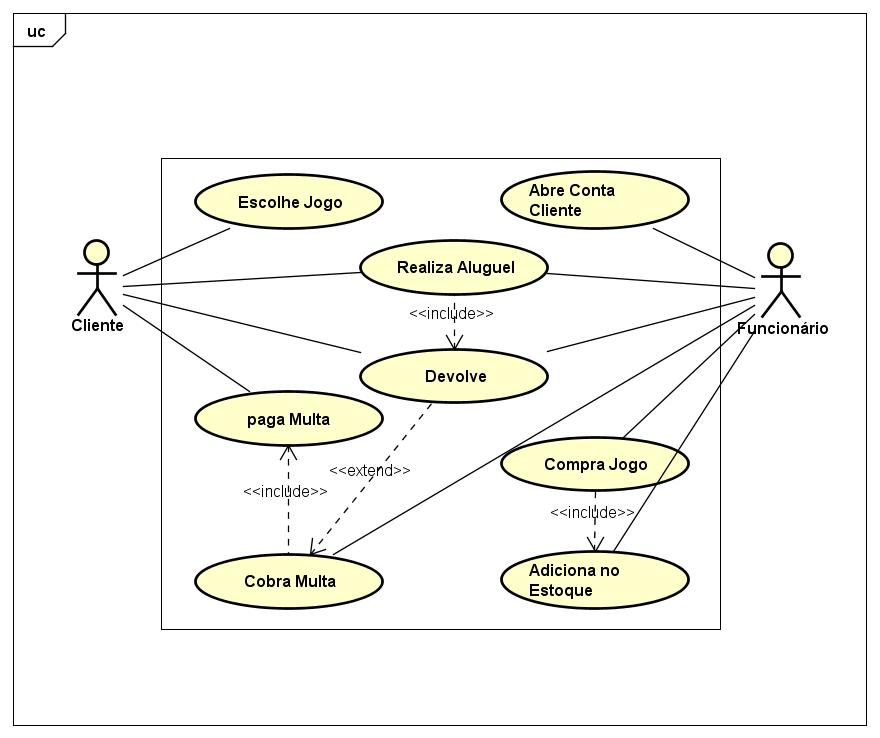
\includegraphics[width=.7\columnwidth]{SistemaDeControleDeLocadoraDeJogos/CasoDeUso.jpg}%
\caption{diagrama de uso para o sistema de controle de Jogos}%
\label{fig:JogosCasosDeUso}%
\end{figure}

\subsubsection{Diagrama de Classes}
\subsubsection{Diagrama de Instâncias}
\subsubsection{Diagrama de Sequências}


\bibliographystyle{plain}
\bibliography{MyLib} 
\end{document} 